\section{Cel pracy}
W tym rozdziale przedstawimy twierdzenie które jest celem całej pracy, czyli twierdzenie o $\varepsilon$-przekształceniach. 
\begin{twie}
    \label{twie:o_prz}
    Zwarta przestrzeń metryczna $X$ ma wymiar pokryciowy co najwyżej $n$ wtedy i tylko wtedy, 
    gdy dla każdego $\varepsilon >0$ istnieje $\varepsilon$-przekształcenie $X$ w wielościan wymiaru co najwyżej $n$.
\end{twie}
Dla ułatwienia, dowodzić je będziemy równolegle z bardzo podobnym twierdzeniem, o $\mathcal{U}$-mapach. 
\begin{twie}
    \label{twie:o_map}
    Zwarta przestrzeń metryczna $X$ ma wymiar pokryciowy co najwyżej $n$ wtedy i tylko wtedy, gdy dla każdego skończonego otwartego pokrycia $\mathcal{U}$ przestrzeni $X$ istnieje $\mathcal{U}$-mapa $X$ w wielościan wymiaru co najwyżej $n$.
\end{twie}


\section{$\varepsilon$-przekształcenie}
Zacznijmy od wprowadzenia definicji $\varepsilon$-przekształcenia oraz $\mathcal{U}$-mapy.
\begin{defi} % 1.10.9
    Niech $\varepsilon>0$, oraz niech $f:X\rightarrow Y$ ciągłe przekształcenie przestrzeni metrycznej $X$ w przestrzeń topologiczną $Y$. 
    Wtedy, powiemy że $f$ jest \emph{$\varepsilon$-przekształceniem}, jeżeli dla każdego punktu w $Y$ średnica przeciwobrazu w tym punkcie jest mniejsza od $\varepsilon$, czyli  $\forall y\in Y \; \diam (f^{-1}(y))<\varepsilon$.
\end{defi}
\begin{przy}
    Weźmy ciąg funkcji ciągłych $f_n:[0,1]\rightarrow[0,1]$ dla $n\ge 2$ z odcinka $[0,1]$ w ten sam odcinek, zdefiniowanych
    \[
    f_n(x) =
    \begin{cases}
        0,                            & x \le \frac{1}{n+1},\\
        \frac{n+1}{n-1}(x-\frac{1}{n+1}), & x \in (\frac{1}{n+1}, \frac{n}{n+1}), \\
        1,                            & x\ge \frac{n}{n+1}.\\
    \end{cases}
    \]
    \begin{figure}[H]
        \centering
        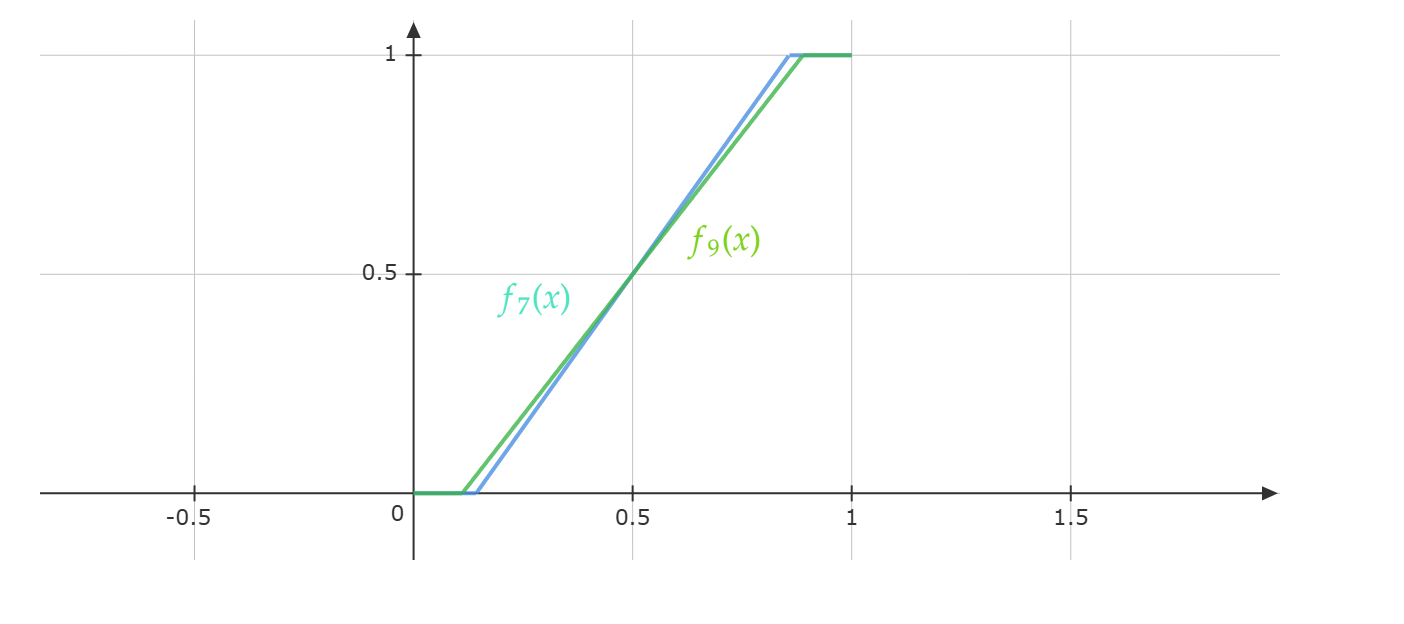
\includegraphics[width=0.8\textwidth]{pictures/eps_funkcja_przyklad.png}
        \caption{$\varepsilon$-przekształcenie}
        \label{fig:eps_2}
    \end{figure}
    Łatwo możemy sprawdzić, że tak zdefiniowane funkcje $f_n$ są odpowiednio $\frac{1}{n}$-przekształceniami (rysunek \ref{fig:eps_2}).
\end{przy}

\begin{defi} % 1.10.8
    Niech $\epsilon$ będzie otwartym pokryciem przestrzeni $X$, oraz niech $f:X\rightarrow Y$ niech będzie ciągłym przekształceniem przestrzeni $X$ w przestrzeń topologiczną $Y$.\\
    Powiemy że $f$ jest \emph{$\mathcal{U}$-mapą}, jeżeli istnieje $\mathcal{V}$ takie  otwarte pokrycie $Y$, że przeciwobraz $f^{-1}(\mathcal{V})$ jest wpisaniem pokrycia $\mathcal{U}$.
\end{defi}

\begin{przy}
    Dla $n\ge 3$, weźmy pokrycie odcinka $(0,1)=I$ 
    \[U=\{(\frac{i-1}{n}, \frac{i+1}{n})\:| \; i=1, \ldots, n-1\}.\]
    Rozpatrzmy otwarty kwadrat $(0,1)\times (0,1)$ i jego dwa pokrycia
    \[U_1 = U\times I\;\;\;\mathrm{oraz}\;\;\; U_2 = I\times U.\]
    Wtedy rzutowanie na pierwszą współrzędną $\pi_1:I^2\rightarrow I$, $\pi_1(x_1,x_2)=x_1$ będzie oczywiście $U_1$-mapą, ale nie będzie $U_2$-mapą. 
\end{przy}

Teraz pokażemy twierdzenie, które pokazuje nam zależność między tymi dwoma definicjami.


\begin{twie}
    \label{twie:map_a_prze}
    Niech $X$ będzie zwartą przestrzenią metryczną, wtedy dla każdego otwartego pokrycia $\mathcal{U}$ przestrzeni $X$, istnieje taka liczba dodatnia $\varepsilon>0$, że każde $\varepsilon$-przekształcenie w przestrzeń Hausdorffa jest też $\mathcal{U}$-mapą.
\end{twie}
\begin{proof}
    Weźmy dowolne otwarte pokrycie $\mathcal{U}$ przestrzeni $X$. Teraz niech $\varepsilon>0$ będzie liczbą Lebesgue'a pokrycia $\mathcal{U}$ - czyli taką wielkością, że dla każdego podzbioru $A\subset X$, jeżeli średnica $\delta(A)$ jest mniejsza od $\varepsilon$, to $A$ zawiera się w którymś elemencie pokrycia $\mathcal{U}$.\\
    Weźmy teraz dowolne $\varepsilon$-przekształcenie $f:X\rightarrow Y$, gdzie $Y$ to przestrzeń Hausdorffa. Pokażemy, że musi ono być również $\mathcal{U}$-mapą.\\
    Zauważmy, że dla każdego elementu $y\in Y$ możemy znaleźć taki element pokrycia $U_y\in \mathcal{U}$, dla którego $f^{-1}(y)\subset U_y$. Z tego że funkcja $f$ jest przekształceniem ciągłym z przestrzeni zwartej w przestrzeń Hausdorffa wiemy, że jest zamknięta na zbiory zamknięte, więc zbiór
    \[V_y = Y\backslash f(X\backslash U_y)\]
    jest oczywiście otwarty. Łatwo możemy sprawdzić, że zachodzi $y\in V_y$, oraz że $f^{-1}(V_y)\subset U_y$. \\
    W takim razie zbiór $\mathcal{V} = \{V_y\}_{y\in Y}$ będzie pokryciem przestrzeni $Y$ spełniającym $f^{-1}(V)$ jest wpisaniem $\mathcal{U}$, co kończy dowód.
\end{proof}
Udowodnimy teraz dwa twierdzenia pomocnicze. 
\begin{twie} % 1.10.11
    \label{twie:1_10_11}
    Jeżeli dla każdego otwartego skończonego pokrycia $\mathcal{U}$ przestrzeni normalnej $X$ istnieje $\mathcal{U}$-mapa w przestrzeń zwartą $Y$ wymiaru co najwyżej $n$, to $\dim X\le n$.
\end{twie}  
\begin{proof}
    Weźmy dowolne otwarte skończone pokrycie $\mathcal{U}$ przestrzeni $X$, oraz niech $f:X\rightarrow Y$ będzie $\mathcal{U}$-mapą w przestrzeń $Y$, $\dim Y\le n$.\\
    Niech $\mathcal{V}$ będzie takim otwartym pokryciem $Y$, że $f^{-1}(\mathcal{V})$ jest wpisaniem $\mathcal{U}$. Teraz skoro $Y$ jest zwarte, to $\mathcal{V}$ ma skończone otwarte wpisanie $\mathcal{V'}$, a korzystając z $\dim Y\le n$ wiemy, że dla $\mathcal{V'}$ możemy znaleźć otwarte wpisanie $\mathcal{W}$, które spełnia $\ord \mathcal{W\le }n$. \\
    Zauważmy teraz, że $f^-1(\mathcal{W})$ też jest skończonym otwartym pokryciem $X$, które jest wpisane w $\mathcal{U}$ i spełnia $\ord f^{-1}(\mathcal{W})\le n$, skąd wynika $\dim X \le n$, co kończy dowód.
\end{proof}

\begin{twie} % 1.10.12
    \label{twie:1_10_12}
    Jeżeli dla każdej liczby $\varepsilon>0$ istnieje $\varepsilon$-przekształcenie zwartej przestrzeni metrycznej $X$ w zwartą przestrzeń $Y$ wymiaru co najwyżej $n$, to $\dim X\le n$.
\end{twie}
\begin{proof}
    Zauważmy, że dowód tego twierdzenia wynika wprost z twierdzeń \ref{twie:1_10_11} oraz \ref{twie:map_a_prze}: \\
    weźmy $\mathcal{U}$-dowolne otwarte pokrycie przestrzeni $X$ i jako $\varepsilon>0$ weźmy liczbę Lebesgue'a tego pokrycia. Teraz wiemy, że możemy znaleźć $\varepsilon$-przekształcenie $f:X\rightarrow Y$ które będzie też $\mathcal{U}$-mapą, więc $\dim X\le n$.
\end{proof}

Zauważmy, że twierdzenia \ref{twie:1_10_12} oraz \ref{twie:1_10_11} są tak naprawdę implikacjami w jedną stronę twierdzeń \ref{twie:o_prz} oraz \ref{twie:o_map}, jeżeli lekko zmodyfikujemy ich treści i zamienimy dowolną przestrzeń zwartą $Y$ wymiaru $\dim Y \le n$ w wielościan wymiaru $n$, dowód będzie przebiegał bardzo podobnie. \\
W takim razie, do dokończenia dowodów, jedyne co zostaje nam pokazać, to że zawsze jesteśmy w stanie takie przekształcenia znaleźć.

\section{Funkcja $\kappa$-kuratowskiego}
\begin{defi}
    Niech $\mathcal{U} = \{U_i \} _{i=1}^k$ będzie skończonym otwartym pokryciem przestrzeni topologicznej $X$ oraz niech $p_1, p_2, \ldots, p_k \in \mathbb{R}^m$ Bedzie ciągiem punktów.\\
    Ciągłe przekształcenie z przestrzeni $X$ w $\mathbb{R}^m$ $\kappa :X\rightarrow R^m$ zdefiniujmy jako
    \[\kappa(x) = \kappa_1(x)p_1+\kappa_2(x)p_2+\cdots+\kappa_k(x)p_k ,\]
    gdzie 
    \[\kappa_i(x) = \frac{\rho(x, X\backslash U_i)}{\sum _{j=1}^k\rho(x, X\backslash U_j)}.\]
    Taką funkcję nazwiemy funkcją \emph{$\kappa$-Kuratowskiego}.
    \cite{kuratowski1933}
\end{defi}
Zauważmy, że w tej definicji może zdarzyć się, że element pokrycia będzie równy całej przestrzeni $X$, czyli $U_i=X$, wtedy we wzorze pojawi się odległość punktu od zbioru pustego. By uniknąć tego problemu, skorzystamy z definicji funkcji $\rho$ zdefiniowanej w \cite{engelking1989}, dla której przyjmujemy $\rho(x, \emptyset)=1$.\\
Zwróćmy uwagę na to, że tak zdefiniowana funkcja jest dobrze określona, jako że jeżeli $x\in X$ należy do $U_i$, to $\rho(x, X\backslash U_i)>0$, za czym idzie 
$\forall x\in X\;\;\sum _{j=1}^k\rho(x, X\backslash U_j)>0$, ponieważ $\mathcal{U}$ jest pokryciem.\\ 
Własnością na którą warto zwrócić uwagę, jest to dla każdego $x\in X$ zachodzi $\sum_{i=1}^{k}\kappa_i(x)=1$, oraz oczywiście wszystkie $\kappa_i(x)\ge 0$.\\
Warto również pokazać, że przekształcenie $\kappa$ rzeczywiście jest ciągłe. To wynika jednak wprost z ciągłości funkcji $\rho(\cdot, A)$ dla ustalonego zbioru $A$, oraz oczywiście z tego, że złożenie funkcji ciągłych również jest funkcją ciągłą.\\

Udowodnimy teraz dwa twierdzenia, pierwsze mówi o przybliżaniu ciągłych przekształceń funkcjami $\kappa$-Kuratowskiego, a drugie jest o własnościach tej funkcji.

\begin{twie} % 1.10.6
    Niech $f:X\rightarrow \mathbb{R}^m$ będzie ciągłym przekształceniem przestrzeni metrycznej $X$ w przestrzeń euklidesową $\mathbb{R}^m$ oraz niech $\delta>0$. \\
    Jeżeli $\mathcal{U} = \{U_i\}_{i=1}^k$ jest otwartym pokryciem $X$, a punkty $p_1, \ldots ,p_k \in R^m$ spełniają
    \[\delta(\{p_i\}\cup f(U_i))<\delta,\]
    to $\kappa$-przekształcenie określone przez $\mathcal{U}$ oraz $p_1, \ldots, p_k$ spełnia 
    \[\rho(f(x), \kappa(x))<\delta\;\;\forall x\in X.\]
\end{twie}
\begin{proof}
    Weźmy $x\in X$, i niech $U_{i_0}, \ldots, U_{i_l}$ będą tymi elementami pokrycia, które zawierają $x$. Teraz, z definicji funkcji $\kappa$ wiemy, że 
    $\kappa_i(x) = 0$ dla wszystkich indeksów poza $i_0, \ldots, i_l$. Z warunku w twierdzeniu dostajemy, że dla $j=0, \ldots, l$ zachodzi
    \[||f(x) - p_{i_j}|| = \rho(f(x), p_{i_j})< \delta,\]
    gdzie $||\cdot ||$ to oczywiście norma. A stąd korzystając z nierówności trójkąta
    \[\rho(f(x), \kappa(x)) = ||f(x) - \kappa(x)|| = \]
    \[||\sum_{i=1}^k \kappa_i(x)\cdot f(x) - \sum_{i=1}^k \kappa_i(x)\cdot p_{i}|| =\]
    \[||\sum_{j=0}^l \kappa_{i_j}(x)\cdot f(x) - \sum_{j=0}^l \kappa_{i_j}(x)\cdot p_{i_j}|| \le\]
    \[\sum_{j=0}^l \kappa_{i_j}(x) \cdot ||f(x)-p_{i_j}||< \delta\cdot\sum_{j=0}^l \kappa_{i_j}(x) = \delta\]
    co kończy dowód.
\end{proof}

\begin{twie} % 1.10.7
    \label{twie:1_10_7}
    Niech $\mathcal{U} = \{U_i\}_{i=1}^k$ będzie otwartym skończonym pokryciem przestrzeni metrycznej $X$, a $\mathcal{N(U)}$ będzie nerwem tego pokrycia o wierzchołkach $p_1, \ldots, p_k\in R^m$. 
    Wtedy, przekształcenie $\kappa$ określone przez pokrycie $\mathcal{U}$ oraz punkty $p_1, \ldots, p_k$ spełnia:
    \[\kappa(X) \subset \mathcal{N(U)}\]
    oraz
    \[\kappa ^{-1}(St_{\mathcal{N(U)}}(p_i))=U_i\;\;\;\;\ \forall i =1, \ldots, k\] 
\end{twie}
\begin{proof}
    Weźmy $x\in X$ oraz niech $U_{i_0}, \ldots, U_{i_l}$ będą elementami pokrycia zawierającymi $x$. Wiemy, że $U_{i_0}\cap  \ldots\cap U_{i_l} \ne \emptyset$ bo oczywiście zawiera element $x$ czyli, z definicji nerwu, sympleks $\Delta (p_{i_0}, \ldots, p_{i_l})$ należy do $\mathcal{N(U)}$. Z własności funkcji $\kappa$ ($\sum _{i=1}^k\kappa_i(x)=1$, $\kappa_i(x)\ge 0) $ możemy pokazać, że $\kappa(x)\in \Delta(p_{i_0}, \ldots, p_{i_l})$, skąd oczywiście $\kappa(x)\in \mathcal{N(U)}$.\\

    Teraz pokażemy drugą równość. Wiemy, że przedstawienie punktów w kompleksie w postaci $\sum_{i=1}^k \lambda_i p_i$ jest jednoznaczne, dostajemy równość
    \[
    \lambda_i (\kappa(x))=\kappa_i(x),
    \]
    a stąd dla każdego $i=1,2,\ldots,k$ zachodzi
    \[ \kappa^{-1}(\St _{\mathcal{N(U)}}(p_i))= \]
    \[ \{x\in X \;:\; \kappa(x)\in \St _{\mathcal(N(U))(p_i)}\}= \]
    \[\{x\in X \;:\; \lambda_i(\kappa(x))>0\}=\]
    \[\{ x\in X \;:\; \kappa_i(x)>0 \} = U_i\]
    co kończy dowód.
\end{proof}

\section{Twierdzenie o $\varepsilon$-przekształceniach}
Możemy w takim razie przejść do dowodu finalnego twierdzenia.
\begin{proof}
    Twierdzenia \ref{twie:o_map}\\ 
    $(\Rightarrow)$\\
    Dla przestrzeni $X$ o wymiarze $\dim X = -1$, czyli przestrzeni pustej, dowód oczywisty. Niech w takim razie przestrzeń $X$ spełnia $0\le \dim X\le n$ oraz niech $\mathcal{U}$ będzie dowolnym skończonym otwartym pokryciem $X$. Teraz, skoro $\dim X\le n$, to możemy znaleźć otwarte wpisanie $\mathcal{V}=\{V_i\}_{i=1}^k$ pokrycia $\mathcal{U}$, spełniające $\ord \mathcal{V}\le n$. Weźmy w takim razie nerw tego pokrycia $\mathcal{N(V)}$, który oczywiście spełnia $\dim \mathcal{N(V)}\le n$, o wierzchołkach $p_1, \ldots, p_k$.\\
    Zauważmy, że $\kappa$-przekształcenie pokreślone przez pokrycie $\mathcal{V}$ oraz punkty $p_1, \ldots, p_k$ jest szukaną $\mathcal{U}$-mapą ponieważ 
    $\{St_{\mathcal{N(V)}}(p_i)\}_{i=1}^k$ jest otwartym pokryciem $\mathcal{N(V)}$, a z twierdzenia \ref{twie:1_10_7} wiemy, że 
    \[\kappa ^{-1}(\{St_{\mathcal{N(V)}}(p_i)\}_{i=1}^k)=\mathcal{V},\]
    co kończy nam tę część dowodu. Pozostaje pokazać implikację w drugą stronę.\\
    $(\Leftarrow)$\\
    Ta implikacja została udowodniona wcześniej w lekko zmodyfikowanym twierdzeniu \ref{twie:1_10_11}.
\end{proof}

\begin{proof} 
    Twierdzenia \ref{twie:o_prz}\\
    $(\Leftarrow)$\\
    Podobnie jak w poprzednim twierdzeniu, tą część udowodniliśmy już wcześniej w \ref{twie:1_10_12}. Pozostaje w takim razie druga implikacja.\\
    $(\Rightarrow)$\\
    Mamy zwartą przestrzeń metryczną $X$ o wymiarze pokryciowym $\dim X\le n$ oraz ustalmy liczbę $\varepsilon>0$. Weźmy pokrycie $\mathcal{U}$ będące skończonym wpisaniem pokrycia $\{ \mathcal{B}(x, \frac{\varepsilon}{3}) \}_{x\in X}$. Z twierdzenia \ref{twie:o_map} wiemy, że możemy znaleźć $\mathcal{U}$-mapę $f:X\rightarrow Y$  przestrzeni $X$ w wielościan wymiaru co najwyżej $n$. Pozostaje w takim razie pokazać, że jest to również $\varepsilon$-przekształceniem. \\
    Wiemy, że możemy znaleźć otwarte pokrycie $\mathcal{V}$ przestrzeni $Y$, dla którego $f^{-1}(\mathcal{V})$ jest wpisaniem $\mathcal{U}$, a z tego oczywiście dostajemy że dla każdego elementu pokrycia $V\in \mathcal{V}$ 
    \[\delta (f^{-1}(V))< \varepsilon\]
    oraz dla każdego elementu $y \in Y$
    \[\delta (f^{-1}(y))< \varepsilon\]
    co kończy dowód.    
\end{proof}

\section{Odwrócone ciągi wielościanów}
Jednym z ważnych wniosków z twierdzenia \ref{twie:o_prz}, jest że klasa zwartych przestrzeni metrycznych o wymiarze pokryciowym co najwyżej $n$, pokrywa się z klasą przestrzeni homeomorficznych do granicy odwróconych ciągów wielościanów o wymiarze co najwyżej $n$. 
\begin{defi}
    Układem odwrotnym, $S = \{X_i, \pi_j^i, N\}$, gdzie $N$ jest zbiorem wszystkich dodatnich liczb całkowitych nazwiemy \emph{odwróconym ciągiem}, często oznaczanym po prostu jako $\{X_i, \pi_j^i\}$. \cite{engelking1989}
\end{defi}
Tutaj $X_i$ są przestrzeniami topologicznymi, a funkcje $\pi _j^i:X_i \rightarrow X_j$ to ciągłe przekształcenia spełniające $\pi _j^i \pi_i^k = \pi _j^k$, oraz $\pi _i^i=\id_{X_i}$.

\begin{defi}
    Element $\{x_i\}_{i\in N}$, $x_i \in X_i$ nazwiemy \emph{nicią} odwróconego ciągu 
    $S = \{X_i, \pi_j^i, N\}$, 
    jeżeli dla każdych indeksów $i, j\in N$, $j\le i$ spełnione jest $\pi _j^i(x_i)=x_j$. Teraz podzbiór przestrzeni $\prod_{i\in N}X_i$, składający się ze wszystkich nici $S$ nazwiemy \emph{granicą odwrotną odwrotnego ciągu $S$} (ozn. $\varprojlim S$).
\end{defi}

\begin{twie}
    Zwarta przestrzeń metryczna $X$ spełnia nierówność $\dim X\le n$ wtedy i tylko wtedy, gdy jest homeomorficzna do granicy odwróconego ciągu wielościanów o wymiarze $\le n$.
\end{twie}
\begin{proof}
    Możemy znaleźć w rozdziale 1.13 w \cite{engelking1995}.
\end{proof}

Pokażemy teraz kilka przykładów pokazujących użycie tego twierdzenia

\begin{przy}
    Pokażemy, że wymiar okręgu jednostkowego jest co najwyżej $1$, poprzez homeomorfizm z granicą ciągu wielokątów. $X_i$ dla $i\ge 2$ to będą obwody $2^i$-kątów foremnych o wspólnych wierzchołkach znajdujących się na tym samym okręgu, a funkcje $\pi_j^j$ - rzut radialny. Wtedy oczywiście dla każdego $i$ spełnione jest $\dim X_i = 1$, więc okrąg, który jest homeomorficzny z granicą tego odwróconego ciągu, również ma wymiar co najwyżej 1.
    \begin{figure}[H]
        \centering
        
\resizebox{0.25\textwidth}{!}{%
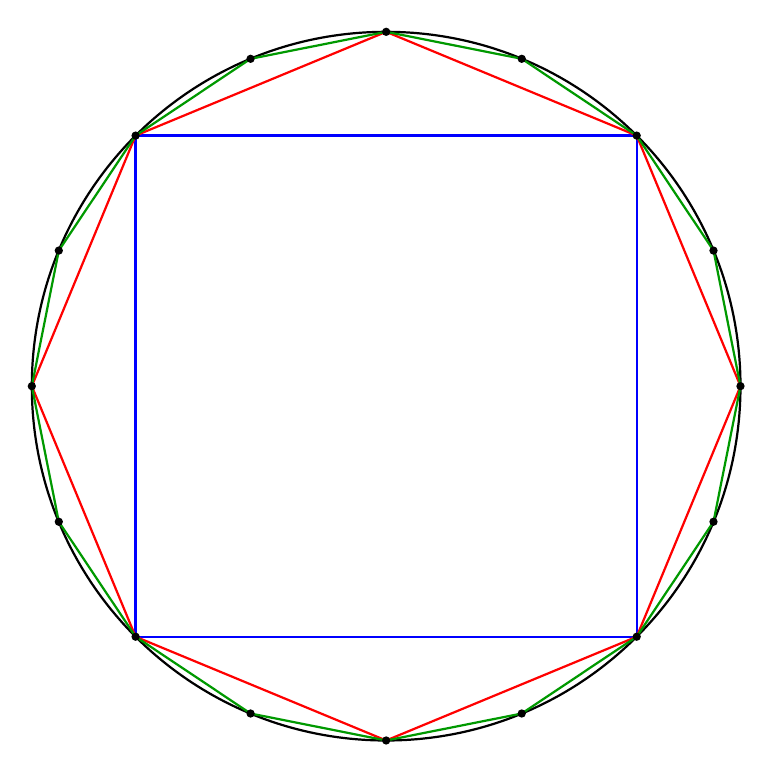
\begin{tikzpicture}[scale=1.5, line width=0.8pt]

% Promien okregu
\def\R{3}

% ---------- Okrag opisany ----------
\draw[black, thick] (0,0) circle (\R);

% ---------- Kwadrat obrocony o 45 stopni ----------
% Wierzcholki kwadratu: katy 45, 135, 225, 315
% Wspolrzedne:
%   45°:  (R*cos45, R*sin45) = (R/sqrt2, R/sqrt2)
%   135°: (-R/sqrt2, R/sqrt2)
%   225°: (-R/sqrt2, -R/sqrt2)
%   315°: (R/sqrt2, -R/sqrt2)
\draw[blue, thick] 
  ({-\R/sqrt(2)},{\R/sqrt(2)}) -- 
  ({\R/sqrt(2)},{\R/sqrt(2)}) -- 
  ({\R/sqrt(2)},{-\R/sqrt(2)}) -- 
  ({-\R/sqrt(2)},{-\R/sqrt(2)}) -- cycle;

% ---------- Foremny osmiokat ----------
% Wierzcholki co 45 stopni: 0, 45, 90, 135, 180, 225, 270, 315
\draw[red, thick] 
  (\R,0) --
  ({\R/sqrt(2)},{\R/sqrt(2)}) --
  (0,\R) --
  ({-\R/sqrt(2)},{\R/sqrt(2)}) --
  (-\R,0) --
  ({-\R/sqrt(2)},{-\R/sqrt(2)}) --
  (0,-\R) --
  ({\R/sqrt(2)},{-\R/sqrt(2)}) -- cycle;

% ---------- Foremny szesnastokat ----------
% Wierzcholki co 22.5 stopni: 0, 22.5, 45, 67.5, 90, ...
\draw[green!60!black, thick] 
  (\R,0) --
  ({cos(22.5)*\R},{sin(22.5)*\R}) --
  ({\R/sqrt(2)},{\R/sqrt(2)}) --
  ({cos(67.5)*\R},{sin(67.5)*\R}) --
  (0,\R) --
  ({cos(112.5)*\R},{sin(112.5)*\R}) --
  ({-\R/sqrt(2)},{\R/sqrt(2)}) --
  ({cos(157.5)*\R},{sin(157.5)*\R}) --
  (-\R,0) --
  ({cos(202.5)*\R},{sin(202.5)*\R}) --
  ({-\R/sqrt(2)},{-\R/sqrt(2)}) --
  ({cos(247.5)*\R},{sin(247.5)*\R}) --
  (0,-\R) --
  ({cos(292.5)*\R},{sin(292.5)*\R}) --
  ({\R/sqrt(2)},{-\R/sqrt(2)}) --
  ({cos(337.5)*\R},{sin(337.5)*\R}) -- cycle;

% ---------- Wierzcholki (kropki) ----------
% Wspolne wierzcholki: co 45 stopni (kwadrat + osmiokat)
\foreach \angle in {0,45,90,135,180,225,270,315} {
  \fill[black] ({\R*cos(\angle)},{\R*sin(\angle)}) circle (1pt);
}
% Dodatkowe wierzcholki szesnastokata: co 22.5 stopni (te, ktorych nie ma wyzej)
\foreach \angle in {22.5,67.5,112.5,157.5,202.5,247.5,292.5,337.5} {
  \fill[black] ({\R*cos(\angle)},{\R*sin(\angle)}) circle (1pt);
}

% % ---------- Srodek okregu ----------
% \fill[black] (0,0) circle (1.5pt);
% \node[below left] at (0,0) {$O$};

% ---------- Etykiety ----------
% \node[blue, below] at (0,-3.5) {kwadrat (obrócony o $45^\circ$)};
% \node[red, below] at (0,-4.0) {ośmiokąt foremny};
% \node[green!60!black, below] at (0,-4.5) {szesnastokąt foremny};
% \node[gray, below] at (0,-5.0) {okrąg opisany};

\end{tikzpicture}
}
        \caption{Rysunek obrazujący.}
        \label{fig:okrag}
    \end{figure}
    
\end{przy}

\begin{przy}
    Pokażemy, że zbiór \emph{Cantora} jest wymiaru 0. \\
    $X_i$ to będą indeksowane od 0 zbiory dyskretne $2^i$-elementowe, a funkcje $\pi _i^{i+1}$ będą określone przez równania $\pi _i^{i+1}(x_{i+1, 2j})= x_{i, j}$, $\pi _i^{i+1}(x_{i+1, 2j+1})= x_{i, j}$. Zauważmy, że dla takiego systemu, możemy znaleźć homeomorfizm między jego granicą a zbiorem cantora w reprezentacji korzystającej z systemu trójkowego: wiemy, że każdą liczbę ze zbioru Cantora jako 
    $\sum _{i=1}^\infty a_i \cdot \frac{1}{3^i}$, gdzie $a_i\in \{0,2\}$. Teraz, elementom każdej przestrzeni $X_i$ przyporządkujemy parami różne elementy $\{0,2\}^i$ tak by funkcje ${\pi}_i^{j}$ były rzutowaniami na pierwsze $i$ współrzędnych. Zauważmy że dla takiego przyporządkowania homeomorfizm między zbiorem Cantora a $\varprojlim \{X_i, \pi _i^j\}$ jest trywialny.
    \begin{figure}[H]
        \centering
        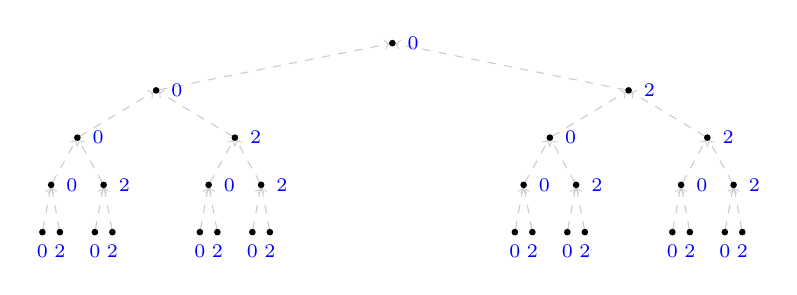
\begin{tikzpicture}[scale=1.0, every node/.style={text=blue}]

\def\ysep{0.6}
\def\rad{1.2pt}
\def\labelshift{2pt}

\newcommand{\bitlabel}[1]{%
  \ifodd#1
    0%
  \else
    2%
  \fi
}

% ---------- definicje współrzędnych ----------
\coordinate (P0-1) at (4.5, 0);

\coordinate (P1-1) at (1.5, -\ysep);
\coordinate (P1-2) at (7.5, -\ysep);

\coordinate (P2-1) at (0.5, -2*\ysep);
\coordinate (P2-2) at (2.5, -2*\ysep);
\coordinate (P2-3) at (6.5, -2*\ysep);
\coordinate (P2-4) at (8.5, -2*\ysep);

\coordinate (P3-1) at (0.1667, -3*\ysep);
\coordinate (P3-2) at (0.8333, -3*\ysep);
\coordinate (P3-3) at (2.1667, -3*\ysep);
\coordinate (P3-4) at (2.8333, -3*\ysep);
\coordinate (P3-5) at (6.1667, -3*\ysep);
\coordinate (P3-6) at (6.8333, -3*\ysep);
\coordinate (P3-7) at (8.1667, -3*\ysep);
\coordinate (P3-8) at (8.8333, -3*\ysep);

\coordinate (P4-1)  at (0.0556, -4*\ysep);
\coordinate (P4-2)  at (0.2778, -4*\ysep);
\coordinate (P4-3)  at (0.7222, -4*\ysep);
\coordinate (P4-4)  at (0.9444, -4*\ysep);
\coordinate (P4-5)  at (2.0556, -4*\ysep);
\coordinate (P4-6)  at (2.2778, -4*\ysep);
\coordinate (P4-7)  at (2.7222, -4*\ysep);
\coordinate (P4-8)  at (2.9444, -4*\ysep);
\coordinate (P4-9)  at (6.0556, -4*\ysep);
\coordinate (P4-10) at (6.2778, -4*\ysep);
\coordinate (P4-11) at (6.7222, -4*\ysep);
\coordinate (P4-12) at (6.9444, -4*\ysep);
\coordinate (P4-13) at (8.0556, -4*\ysep);
\coordinate (P4-14) at (8.2778, -4*\ysep);
\coordinate (P4-15) at (8.7222, -4*\ysep);
\coordinate (P4-16) at (8.9444, -4*\ysep);

% ---------- strzałki dziecko -> rodzic, jasne, przerywane ----------
\tikzset{
  arrowstyle/.style={
    ->,
    draw=gray!40,
    dashed,
    shorten >=1pt,
    shorten <=1pt,
    thin
  }
}

% Krok 1 -> Krok 0
\draw[arrowstyle] (P1-1) -- (P0-1);
\draw[arrowstyle] (P1-2) -- (P0-1);

% Krok 2 -> Krok 1
\foreach \c in {1,2} {
  \draw[arrowstyle] (P2-\c) -- (P1-1);
  \draw[arrowstyle] (P2-\the\numexpr\c+2\relax) -- (P1-2);
}

% Krok 3 -> Krok 2
\foreach \c in {1,2,3,4} {
  \draw[arrowstyle] (P3-\the\numexpr2*\c-1\relax) -- (P2-\c);
  \draw[arrowstyle] (P3-\the\numexpr2*\c\relax) -- (P2-\c);
}

% Krok 4 -> Krok 3
\foreach \c in {1,...,8} {
  \draw[arrowstyle] (P4-\the\numexpr2*\c-1\relax) -- (P3-\c);
  \draw[arrowstyle] (P4-\the\numexpr2*\c\relax) -- (P3-\c);
}

% ---------- punkty i etykiety ----------
\foreach \x [count=\i from 1] in {4.5} {
  \fill (\x, 0) circle (\rad);
  \node[right=\labelshift] at (\x, 0) {\scriptsize \bitlabel{\i}};
}
\foreach \x [count=\i from 1] in {1.5, 7.5} {
  \fill (\x, -\ysep) circle (\rad);
  \node[right=\labelshift] at (\x, -\ysep) {\scriptsize \bitlabel{\i}};
}
\foreach \x [count=\i from 1] in {0.5, 2.5, 6.5, 8.5} {
  \fill (\x, -2*\ysep) circle (\rad);
  \node[right=\labelshift] at (\x, -2*\ysep) {\scriptsize \bitlabel{\i}};
}
\foreach \x [count=\i from 1] in {0.1667, 0.8333, 2.1667, 2.8333, 6.1667, 6.8333, 8.1667, 8.8333} {
  \fill (\x, -3*\ysep) circle (\rad);
  \node[right=\labelshift] at (\x, -3*\ysep) {\scriptsize \bitlabel{\i}};
}
\foreach \x [count=\i from 1] in {
  0.0556, 0.2778, 0.7222, 0.9444,
  2.0556, 2.2778, 2.7222, 2.9444,
  6.0556, 6.2778, 6.7222, 6.9444,
  8.0556, 8.2778, 8.7222, 8.9444
} {
  \fill (\x, -4*\ysep) circle (\rad);
  \node[below=1pt] at (\x, -4*\ysep) {\scriptsize \bitlabel{\i}};
}

\end{tikzpicture}
        \caption{Funkcje $\pi ^{i+1}_i $ oraz system trójkowy.}
        \label{fig:cantor}
    \end{figure}
\end{przy}

\begin{przy}
    W podobny sposób możemy pokazać że wymiar pokryciowy \emph{dywanu sierpińskiego} jest równy 1.
\end{przy}